\documentclass{article}
\usepackage[top=.4in, bottom=.2in, left=.4in, right=.4in]{geometry}
\usepackage{hyperref}
\usepackage{graphicx}
\usepackage{csquotes} %for quotes
\usepackage{amsmath}
\usepackage{setspace}
\usepackage{float}
\usepackage{caption}
\usepackage[font=small, labelfont=bf]{subcaption}
\usepackage{lscape} %landscape
\usepackage[inline]{enumitem}
\renewcommand{\familydefault}{\sfdefault} %change font
\title{Cell classification by applying graphlets on HiC data}
\author{Behnam Rasoolian  \and Liangliang Xu \and Zheng Zhang}
\date{}
\begin{document}
\fontsize{11pt}{13pt}\selectfont
\pagenumbering{gobble}
\setlength{\parindent}{0pt}
\maketitle
\section{Motivation}
In this study, we plan to find dissimilarities between normal cells and cancerous cells,
in terms of the 3D structure of their chromosomes. This is done through
investigating HiC contact maps. 
We suspect that there are systematic differences between how chromosomes are structured
between normal cells and cancerous cells.
\section{Background}
The cell of a eukaryotic species forms a multi-granularity genome structure
in order to compactly store a very long genomic 
DNA sequence in its small nucleus. The following describes the genome
structure in the order of decreasing granularity
\begin{enumerate*}
    \item[(1)] A \textbf{nucelotide} is the building block of
        DNA. There are 4 types of nucleotides: 
        C, G, A and T. 
    \item[(2)] Each pair of nucleotides in the DNA are called a \textbf{base}.
        A kilo-base is a group of 1000 bases.
    \item[(3)] thousands of bases join together to form \textbf{gene loci}.
    \item[(4)] A number of loci then fold into a large
        independent physical structure called \textbf{chromosome}.
\end{enumerate*}

One or more chromosomes interact to constitute the dynamic
\textbf{three-dimensional (3D) conformation} of the entire genome of a cell. 

Ideally, it is desirable to compare these 3D conformation of 
cell in order to make such comparisons.
However, the main challenge that we face is that 
3D structure of a cell is not readily available but there has been
efforts at its characterization:
In other to find dissimilarities in the 3D structure of 
chromosomes, we use HiC dataset.
The HiC method
captures interactions between 
chromosomal fragments in kilobase resolution. Based on HiC data, an
\textit{interaction frequency (IF) } matrix can be developed between \textit{loci} at a desired resolution.
A cell ${IF}_{ij}$ in an interaction frequency matrix captures the number of interaction detected
in HiC dataset between locus $i$ and locus $j$ in the genome.
An interaction matrix can be used to develop both inter- and intra-chromosomal interaction matrices.
\textit{We believe differences in interaction matrices can be found between normal cells and cancerous ones.}

Graphlet comparison is a novel method used to compare large networks in order to
find local similarities in them.
Given a graph $G$, \textbf{fragment} are connected subgraphs $G$.
\textbf{Motifs} are fragments that occur with a frequency much higher than
that occuring in a randomly generated graph.
Given a graph $G(V, E)$ and $S \subseteq V$, then $G'(S, E')$
is an \textbf{induced graphs} iff $E' = \{(u, v) | u, v \in V \text{ and } 
(u, v) \in E \rightarrow (u, v) \in E'\}$.
\textbf{Graphlets} are arbitrary, induced fragments.
An edge is the only two-node graphlet.
\textbf{Orbits} are sets of all nodes in a graphlet that can be
swapped with each other while not changing the graph.
Orbits are ``topographically similar'' to each other.

A \textbf{signature} or \textbf{signature vector} of a node in graph $G$ is
73-dimensional vector $\mathbf{s}^T
= [s_0, s_2, ..., s_{72}]$ where $s_i$ denotes the number of nodes in
the network that are part of an orbit $i$ in G. 
\section{Data and Methods}
We have HiC itra- and inter-chromosomal interaction matices for 4
types of cells, one of which is normal and 
the other three are cancer cells. We will extract signature vectors
of size 73 for each loci in each chromosome. leading to a $23 \times 73$
matrix for each loci. Assuming there are 
$n_i$ loci in each chromosome (i = 1 ... 23),
it would lead to an $N \times P \times M$ matrix
where $N$ is $\sum_{i=1}^{23} {n_i}$ and $P$ and $M$ 
are 23 and 73 respectively. By estimating
$n_i$ to be 100 on average, we expect the
size of the input ($N$) to be $2000$.
We will use the normal cell data and two of the cancer cell 
data in training phase, and use the fourth cell type to
validate the results. In summary, we have 3 categories: normal, 
cancer type I, and cancer type II. The problem is, given
a $23 * 73$ contact graphlet matrix, does it belong to
a normal cell or cancerous cell.
In terms of methods, we plan to start with standard
VGG-Network. We will have to go towards more complicated 
networks in the case of poor results. We will be open
to exploring various architectures and pick one that 
 fits the data better.
\section{Appendix}
\begin{figure}[H]
    \centering
    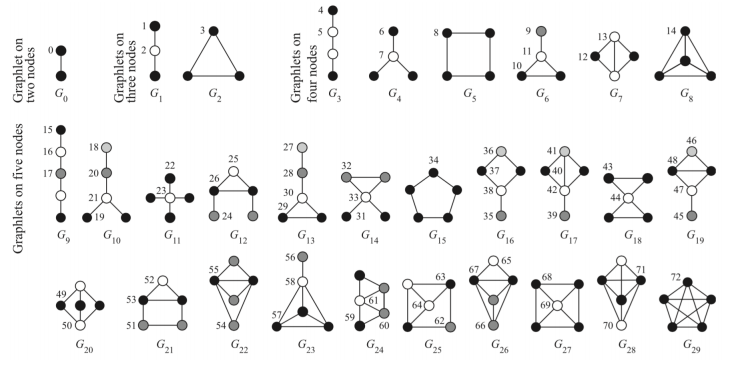
\includegraphics[scale=.5]{graphlets.png}
    \caption{All 30 undirected two- to five-node graphlets
    with 73 orbits.}
    \label{fig:graphletsAndOrbits}
\end{figure}

\bibliography{lit}
\bibliographystyle{unsrt}
\end{document}
